\documentclass[11pt,a4paper]{article}
\usepackage[a4paper,margin=2.3cm]{geometry}
\usepackage{graphicx}
\usepackage{booktabs}
\usepackage{amsmath}
\usepackage{xcolor}
\usepackage{caption}
\usepackage[colorlinks=true,linkcolor=blue!60!black,urlcolor=blue!60!black,citecolor=blue!60!black]{hyperref}
\captionsetup{font=small,labelfont=bf}
\graphicspath{{assets/figs/}}
\definecolor{codebg}{RGB}{246,246,248}
\usepackage{fancyvrb}
\newcommand{\arm}[1]{\textsc{#1}}

\title{\bfseries When Does Intermediate Reward Actually Help?\\
\large Outcome-only credit assignment vs.\ explicit progress supervision\\
for multi-turn LLM search agents --- Research Proposal with Preliminary Results}
\author{Xiaoxuan Lei}
\date{July 16, 2026 \quad (project \texttt{Agentic-RL-CA}, status: Wave~1 complete, Wave~2 in flight)}

\begin{document}
\maketitle

\begin{abstract}
Reinforcement learning for multi-turn LLM agents almost always optimizes a \emph{sparse outcome
reward}: one scalar at the end of a trajectory. Whether an agent benefits from an additional
\emph{intermediate reward signal} --- supplied by an explicit reward model, a privileged
verifiable heuristic, or recovered implicitly by the credit-assignment (CA) machinery of the RL
algorithm itself --- remains unresolved, and published comparisons rarely control for reward
density, compute, or seeds. We propose a controlled study on the Search-R1 question-answering
task: a Qwen3-1.7B agent that interleaves reasoning, search-engine calls, and a final answer over
up to 4 turns (8 in a stress test). We compare seven credit-assignment arms spanning implicit
reward decomposition (token- and turn-level critics; group-relative estimators GRPO/GiGPO/HCAPO)
against explicit progress supervision (a privileged answer-exposure step reward, B1) and a
density-matched shuffled control (B1-shuffle) that uniquely separates the reward's
\emph{information content} from its \emph{optimization effects}. Preliminary results (Wave 0--1,
9 completed or near-complete 500-step runs) show: (i) all arms clear the untrained baseline
(0.225 macro-EM) by a wide margin, with outcome-only group-relative methods leading (GiGPO
$\approx$0.41 val macro-EM, GRPO 0.391 val / 0.395 on the full 51{,}713-question test set);
(ii) explicit progress reward so far adds \emph{no} value over its shuffled control --- the
control currently \emph{beats} it on matched seeds --- consistent with a reward-density rather
than content effect; and (iii) a reproducible late-training instability (response-truncation
runaway) afflicts the critic-based arms, most severely the content-bearing B1 arm, while both
shuffle runs stay clean. We outline the pre-registered analyses (third seeds, 8-turn horizon,
per-dataset multi-hop subgroup, and a Monte-Carlo credit-alignment diagnostic) that will settle
the hypotheses.
\end{abstract}

\section{Motivation}

Agentic RL fine-tuning of LLMs --- tool use, web research, multi-step reasoning --- is
bottlenecked by \textbf{credit assignment}: the outcome reward arrives only after a sequence of
interdependent decisions. The community's responses fall into two families that are rarely
compared under matched conditions:

\begin{enumerate}
  \item \textbf{Implicit reward models.} The RL algorithm itself decomposes the outcome reward:
  a learned value network (token-level or turn-level critic) is, functionally, an implicit
  per-step reward model; group-relative estimators (GRPO and its turn-aware descendants GiGPO,
  HCAPO) sidestep the critic but still implicitly assign per-step credit through grouped
  baselines and anchor-state matching.
  \item \textbf{Explicit intermediate rewards.} A process/progress reward is injected at each
  step --- from a trained process reward model (PRM), a prompted LLM judge, or a verifiable
  domain heuristic.
\end{enumerate}

The central question of this proposal is \textbf{when the second family adds value beyond the
first}, and whether apparent gains from intermediate rewards survive a control that matches
their density and magnitude but destroys their timing/content. This control --- rarely run in
the literature --- is the experiment's key instrument.

\section{Hypotheses}

\begin{itemize}
  \item \textbf{H1 (granularity).} Turn-level credit (one credit unit per agent action) is a
  better-matched inductive bias than token-level credit for multi-turn agents; it should not
  underperform token-level PPO at matched compute.
  \item \textbf{H2 (implicit recovery).} Outcome-only group-relative CA can recover useful
  intermediate credit without any explicit step reward; measured not only by final accuracy but
  by a quantitative credit-alignment diagnostic (assigned credit vs.\ Monte-Carlo continuation
  value, Sec.~\ref{sec:remaining}).
  \item \textbf{H3 (content vs.\ density --- the core hypothesis).} If explicit progress
  supervision helps through its \emph{information content}, a privileged step reward (B1) must
  beat a density-matched shuffled control (B1-shuffle). If B1 $\approx$ B1-shuffle $>$ B0
  (sparse), the benefit is an optimization/density effect that any well-shaped dense signal ---
  including a contentless one --- provides. Preliminary reading: the latter.
  \item \textbf{H4 (horizon scaling).} Any content benefit should grow with task horizon and
  difficulty (multi-hop questions; 8-turn budget), where progress information has more room to
  discriminate.
  \item \textbf{H5 (scalable evaluator, staged).} A prompted step evaluator can approximate the
  privileged signal only if H3 shows content matters; H5 is gated on H3's outcome.
\end{itemize}

\section{Experimental design}

\subsection{Task, dataset, and reward}

\textbf{Task.} Search-R1 protocol: the agent answers open-domain questions by interleaving
\texttt{<think>} reasoning with either a \texttt{<search>query</search>} call to a retriever or
a final \texttt{<answer>...</answer>}, for up to 4 turns (main protocol) or 8 turns (stress
test). Retrieval is dense e5 over the 2018 Wikipedia dump (wiki-18, 61\,GB FAISS index), top-3
passages per query, served by a co-located retrieval server.

\textbf{Training data.} The standard Search-R1 training mixture --- Natural Questions +
HotpotQA training splits (HF \texttt{PeterJinGo/nq\_hotpotqa\_train}, $\sim$170k questions) ---
preprocessed by the versioned pipeline in the repository. Validation during training uses a
fixed stratified 2{,}048-question subset (\texttt{val\_2048}); final evaluation is the full
paper-protocol test set: \textbf{51{,}713 questions over 7 datasets} (NQ, TriviaQA, PopQA
single-hop; HotpotQA, 2WikiMultihopQA, MuSiQue, Bamboogle multi-hop), greedy decoding, exact
match (EM).

\textbf{Outcome reward.} Rule-based EM on the final answer (1/0), with a small invalid-action
penalty. No learned reward model anywhere in the core tier --- by design, so that the
\emph{only} intermediate signal is the one we inject and control.

\textbf{Model.} Qwen3-1.7B (thinking mode, 2{,}048-token responses, 4{,}096-token prompts),
identical across all arms; batch 256, group size 5, 500 PPO steps, identical LR/KL settings.
A pre-registered feasibility gate on the \emph{untrained} model (nonzero EM floor, valid-action
rate $\geq$90\%, search-invocation rate $\geq$50\%, reward variance within rollout groups)
passed at 1.7B, so the fleet stays at this scale (fallback: Qwen3-4B).

\subsection{Conditions: a reward-model taxonomy}

\begin{table}[h]
\centering\small
\begin{tabular}{lllp{5.6cm}}
\toprule
Arm & Estimator & Critic & Where the ``reward model'' lives \\
\midrule
\arm{token-PPO}   & GAE (token)      & yes & implicit: token-level value network \\
\arm{turn-PPO/B0} & GAE (turn)       & yes & implicit: turn-level value network \\
\arm{token-GRPO}  & GRPO             & no  & implicit: group-relative outcome baseline \\
\arm{GiGPO}       & GiGPO            & no  & implicit: episode + anchor-state grouped baselines \\
\arm{HCAPO}       & HCAPO            & no  & implicit: hindsight-conditioned advantage (Wave 2) \\
\arm{B1}          & GAE (turn) + step reward & yes & \textbf{explicit}: privileged answer-exposure signal, $+0.2$ the first turn whose retrieved passages contain the gold answer \\
\arm{B1-shuffle}  & GAE (turn) + shuffled step reward & yes & \textbf{explicit, contentless}: B1's rewards re-assigned uniformly to another non-terminal search turn --- matched count and magnitude, destroyed timing \\
\bottomrule
\end{tabular}
\caption{Core arms. B1 is deliberately \emph{privileged and verifiable} (it peeks at the gold
answer) --- an upper-bound proxy for a perfect progress reward model, free of judge noise. The
shuffled control isolates information content from reward density. A prompted-judge arm
(B2-lite) is staged behind H3.}
\end{table}

\textbf{Pre-registered decision rules} (fixed before any curve was seen): primary comparison =
fixed-budget final checkpoint; sample-efficiency = validation AUC; best-val checkpoint reported
but never the headline. RQ3 is judged on per-seed final-EM and val-AUC deltas with seed ranges
(2--3 seeds per arm), plus a paired per-dataset breakdown with the multi-hop subgroup
pre-registered as the mechanism readout. Interpretation grid: B1 $>$ shuffle $\approx$ B0
$\Rightarrow$ content matters; B1 $\approx$ shuffle $>$ B0 $\Rightarrow$ density effect;
all $\approx$ $\Rightarrow$ this signal does not help at this horizon.

\section{Preliminary results}

Nine 500-step runs are complete or near-complete (Wave 0--1 + partial Wave 2); three third-seed
runs and the 8-turn stress test are in flight. Untrained baseline: 0.225 val macro-EM.

\begin{figure}[h]
\centering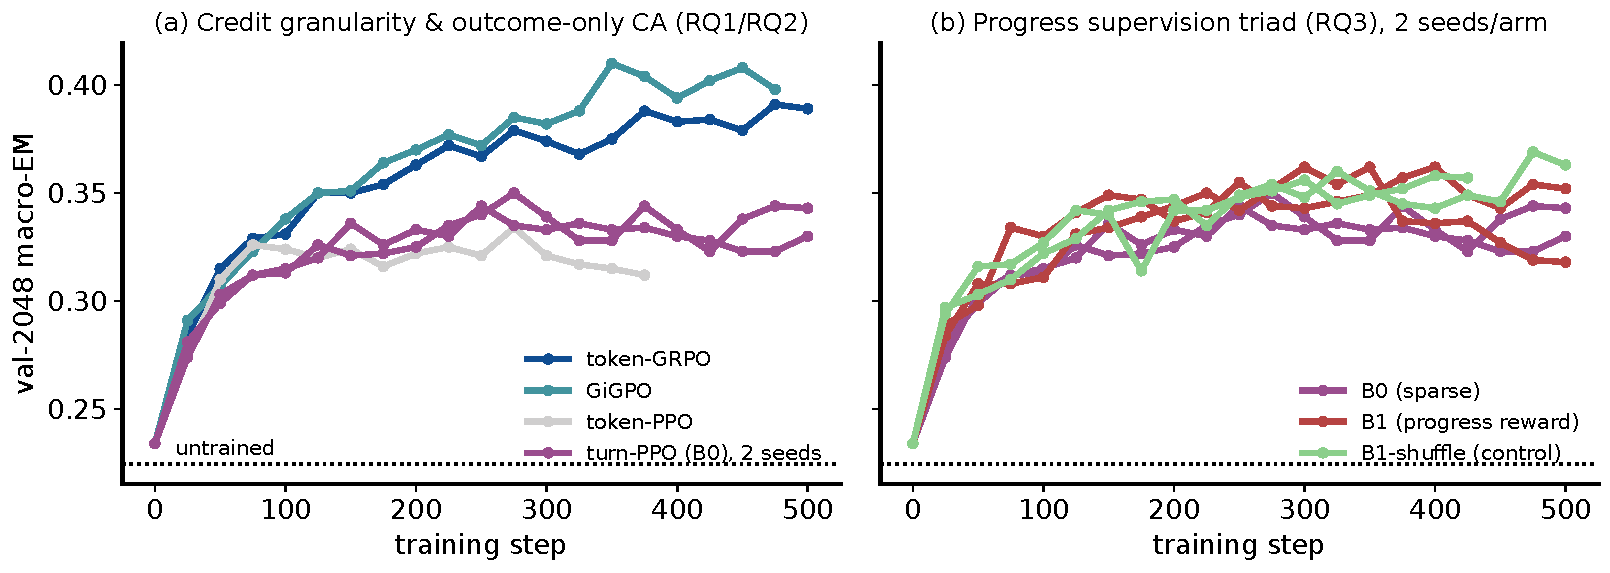
\includegraphics[width=\textwidth]{fig_learning_curves.pdf}
\caption{Validation macro-EM (2{,}048 fixed questions, greedy, every 25 steps).
\textbf{(a)} Outcome-only group-relative methods lead: GiGPO (still training, best 0.410)
tracks above token-GRPO (final 0.391); both critic-based PPO arms plateau near 0.33--0.34;
token-PPO is weakest. \textbf{(b)} The RQ3 triad at two seeds per arm: the three conditions are
statistically inseparable for most of training; late-run divergence is driven by the
instability in Fig.~\ref{fig:trip}.}
\label{fig:curves}
\end{figure}

\begin{figure}[h]
\centering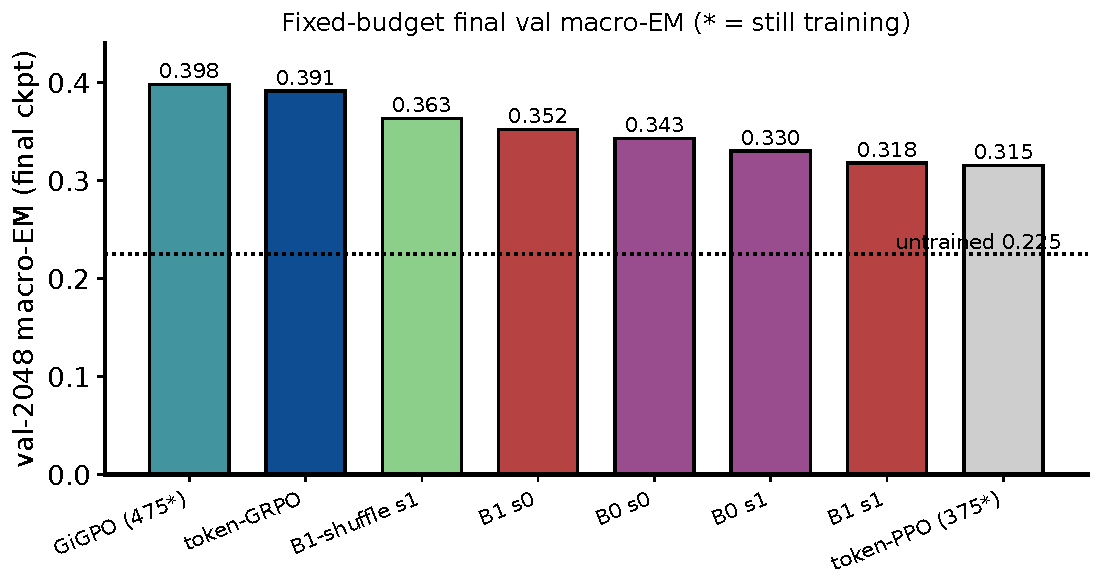
\includegraphics[width=0.72\textwidth]{fig_final_bars.pdf}
\caption{Fixed-budget final val macro-EM (the pre-registered primary comparison). The wave-0
GRPO checkpoint scores \textbf{0.3951 macro-EM on the full 51{,}713-question test set}
(0.4993 single-hop / 0.3170 multi-hop), within $+0.004$ of its val-2048 proxy --- validating
the proxy. Seed pairs: B0 0.343/0.330, B1 0.352/0.318, B1-shuffle 0.363/(s0 running at 0.358).}
\label{fig:bars}
\end{figure}

\begin{figure}[h]
\centering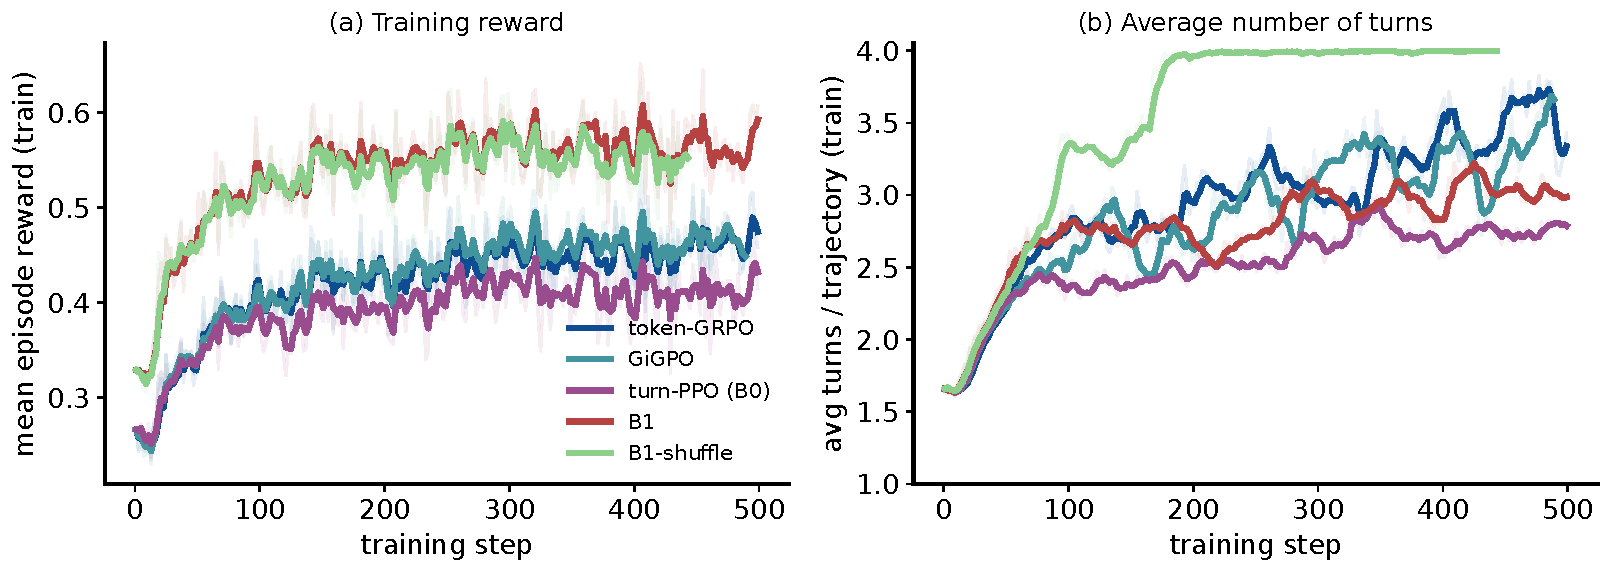
\includegraphics[width=\textwidth]{fig_reward_turns.pdf}
\caption{Training dynamics (seed-0 arms; EMA-smoothed). \textbf{(a)} Mean episode reward.
B1/B1-shuffle sit higher by construction (their reward includes the $+0.2$ step bonus).
\textbf{(b)} Average turns per trajectory grows from $\sim$1.7 to $\sim$3 across all arms ---
agents learn to search more before answering. Notably, the \emph{shuffled} step-reward arm
saturates the 4-turn budget entirely: a contentless dense reward on search turns teaches
``search more,'' not ``search better'' --- yet loses nothing in accuracy, foreshadowing the
density reading of H3.}
\label{fig:dyn}
\end{figure}

\begin{figure}[h]
\centering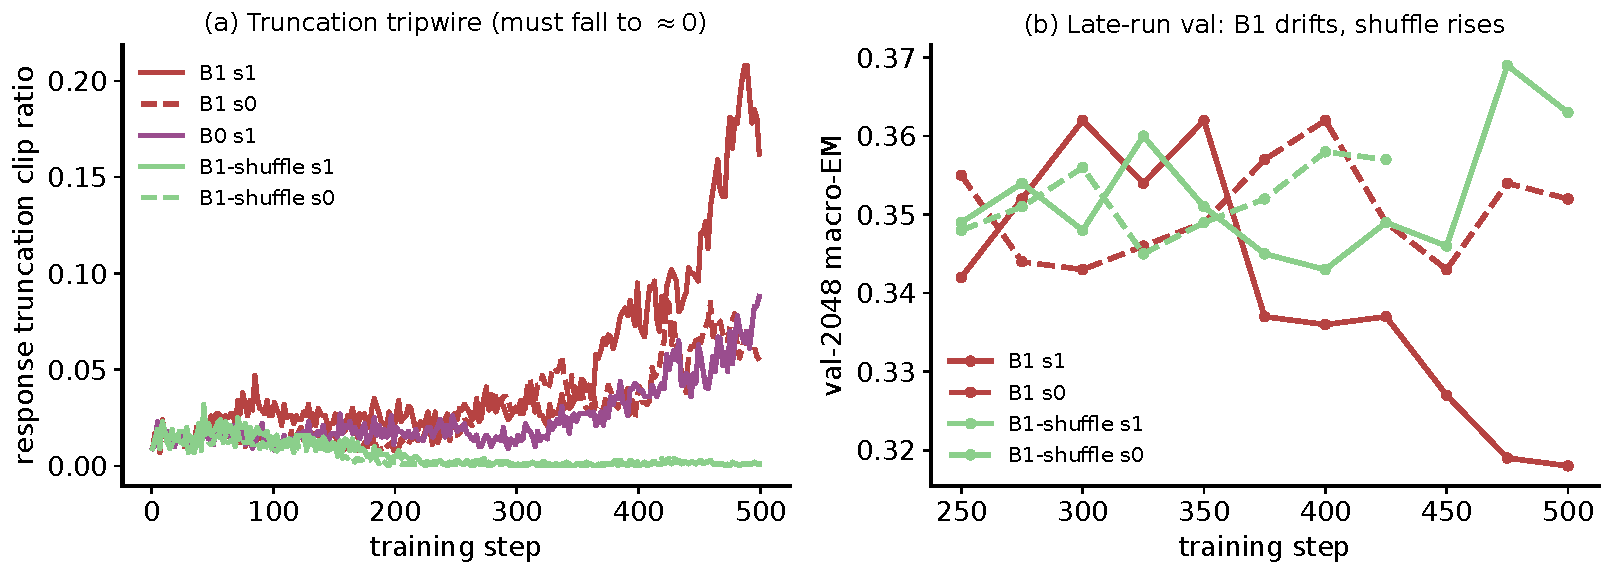
\includegraphics[width=\textwidth]{fig_tripwire.pdf}
\caption{The main preliminary \emph{mechanistic} finding. \textbf{(a)} Response-truncation rate
(fraction of turns hitting the 2{,}048-token cap; must fall to $\approx$0 in a healthy run).
Every critic-based arm drifts upward late in training; the content-bearing B1 seed-1 run runs
away (0.21 by step 500) and its validation accuracy collapses in lockstep, \textbf{(b)}. Both
B1-shuffle seeds stay at $\approx$0 truncation and \emph{rise} late. The explicit progress
reward is implicated in destabilizing generation length; the density-matched control is not.}
\label{fig:trip}
\end{figure}

\subsection{Interim readings}

\begin{enumerate}
  \item \textbf{H1 (granularity):} supported so far --- turn-PPO (0.343/0.330) $\geq$ token-PPO
  ($\sim$0.315, still training) at matched config, though both trail the critic-free arms.
  \item \textbf{H2 (implicit recovery):} strongly supported on accuracy --- GiGPO and GRPO lead
  the table without any intermediate reward. The credit-alignment diagnostic will test whether
  they also assign \emph{correct} intermediate credit.
  \item \textbf{H3 (content vs.\ density):} at 2/2/2 seeds, the pre-registered step-150 window
  readout gave shuffle$-$B0 positive on both seeds and B1$-$shuffle straddling zero; at final
  checkpoints B1-shuffle (0.363) currently \emph{beats} B1 (0.352/0.318) while suffering none
  of its instability. Interim call: \textbf{reward-density/optimization effect, not
  progress-content supervision} --- pending third seeds and val-AUC.
  \item \textbf{Stability as a first-class finding:} the truncation tripwire (Fig.~\ref{fig:trip})
  reproduces across 4/4 critic arms and never in the 3 clean shuffle/GiGPO runs monitored at the
  same wall-clock; the formal report will treat late-training length instability as a cost of
  this class of explicit step reward.
\end{enumerate}

\section{Remaining work}
\label{sec:remaining}

(i) Third seeds for the RQ3 triad (in flight) to tighten the pre-declared seed ranges;
(ii) the \textbf{8-turn horizon stress test} (required; first run launched) --- H4's direct
test, where shuffle has more eligible turns and content has more room to matter;
(iii) HCAPO, GiGPO/GRPO second seeds (wrappers staged);
(iv) the \textbf{credit-alignment diagnostic}: for logged trajectories, estimate each prefix's
Monte-Carlo continuation value $\hat V(s_t)$ by resuming from snapshots under the same
checkpoint, and compare each method's assigned turn credit against
$\Delta\hat V_t = \hat V(s_{t+1})-\hat V(s_t)$ (pooled Spearman, bootstrap CIs) --- upgrading
H2 from a benchmark claim to a measurement of credit fidelity;
(v) full-set evals of all pre-registered final checkpoints;
(vi) B2-lite (prompted step evaluator) only if the third seeds overturn the density reading.

\appendix
\section{Example trajectory (trained GRPO agent, full-set eval, EM = 1)}

\begin{Verbatim}[fontsize=\footnotesize,frame=single]
QUESTION: Who delivered their famous 'The Lady's Not For Turning' speech
          in October 1980?

TURN 1  <search>who delivered their famous 'The Lady's Not For Turning'
        speech in October 1980</search>
        <information>Doc 1: "The lady's not for turning" ... was a phrase
        used by Margaret Thatcher, then Prime Minister, in her speech to
        the Conservative Party Conference on 10 October 1980. ...</information>

TURN 2  <search>who delivered the 'The Lady's Not For Turning' speech in
        1980</search>
        <information>Doc 1: ... Margaret Thatcher, then Prime Minister ...
        (confirmatory retrieval)</information>

TURN 3  <think>... Doc 1 and Doc 2 mention Margaret Thatcher. She was the
        Prime Minister at that time. The speech was delivered at the
        Conservative Party Conference on October 10, 1980. ... I don't see
        any conflicting information.</think>
        <answer>Margaret Thatcher</answer>          --> outcome reward 1.0
\end{Verbatim}

\noindent Under \arm{B1}, turn 1 would additionally receive the $+0.2$ answer-exposure step
reward (first retrieval containing ``Margaret Thatcher''); under \arm{B1-shuffle} that same
$+0.2$ would be re-assigned uniformly among turns 1--2. Redundant confirmatory searches as in
turn 2 are exactly the behavior the average-turns saturation of Fig.~\ref{fig:dyn}b amplifies.

\vspace{0.5em}
\noindent\textbf{Reproducibility.} Figures: \texttt{assets/extract\_metrics.py} +
\texttt{assets/build\_figures.py} (CSV per run under \texttt{assets/csv/}); training logs,
ledger, and the append-only decision log live in the project repository
(\texttt{Agentic-RL-CA}, branch \texttt{agentic-rl-ca}); pre-registration in
\texttt{docs/plan.md}.

\end{document}
